\documentclass[11pt]{article}

% =========================
% Packages
% =========================
\usepackage[margin=0.78in]{geometry}
\usepackage{amsmath,amssymb,amsfonts,mathtools}
\usepackage{booktabs,array,tabularx,longtable,multirow}
\usepackage{enumitem}
\usepackage[most]{tcolorbox}
\usepackage{xcolor}
\usepackage{fancyhdr}
\usepackage{titlesec}
\usepackage{hyperref}
\usepackage{lastpage}
\usepackage{setspace}
\usepackage{tikz}
\usepackage{pgfplots}
\usepackage{needspace}
\usepackage{caption}
\usepackage{multicol}
\usepackage{graphicx}
\usepackage{amsthm}
\usepackage{mathrsfs}
\usepackage{bm}
\usepackage{float}
\usetikzlibrary{calc,arrows.meta,positioning,decorations.pathreplacing}

\pgfplotsset{compat=1.18}
\setstretch{1.14}
\setlength{\parindent}{0pt}
\setlength{\parskip}{0.45em}
\setlist[itemize]{leftmargin=1.8em}
\setlist[enumerate]{leftmargin=2em}

% =========================
% Colors
% =========================
\definecolor{novelPurple}{RGB}{98,54,255}
\definecolor{novelPurpleDark}{RGB}{72,34,204}
\definecolor{novelPurpleLight}{RGB}{243,239,255}
\definecolor{novelPurpleLine}{RGB}{165,135,255}
\definecolor{npgray}{RGB}{78,78,78}
\definecolor{softgray}{RGB}{246,246,250}
\definecolor{softlav}{RGB}{249,247,255}
\definecolor{greencheck}{RGB}{24,128,88}
\definecolor{warmred}{RGB}{188,54,54}
\definecolor{nporange}{RGB}{223,121,36}
\definecolor{npgreen}{RGB}{67,142,103}
\definecolor{npred}{RGB}{180,54,54}

% =========================
% Hyperref
% =========================
\hypersetup{
    colorlinks=true,
    linkcolor=novelPurpleDark,
    urlcolor=novelPurpleDark,
    citecolor=novelPurpleDark
}

% =========================
% Header / Footer
% =========================
\pagestyle{fancy}
\fancyhf{}
\fancyhead[L]{\textbf{Novel Prep Learning Center}}
\fancyhead[R]{\textbf{AP Calculus AB/BC --- Unit 7}}
\fancyfoot[C]{\textcolor{novelPurpleDark}{\thepage\ /\ \pageref{LastPage}}}
\renewcommand{\headrulewidth}{0.4pt}
\renewcommand{\footrulewidth}{0pt}

% =========================
% Numbering / TOC
% =========================
\setcounter{secnumdepth}{3}
\setcounter{tocdepth}{3}

% =========================
% Section styles
% =========================
\titleformat{\section}
{\Large\bfseries\color{novelPurpleDark}}{\thesection.}{0.6em}{}

\titleformat{\subsection}
{\large\bfseries\color{novelPurple}}{\thesubsection.}{0.6em}{}

\titleformat{\subsubsection}
{\normalsize\bfseries\color{novelPurpleDark}}{\thesubsubsection.}{0.6em}{}

% =========================
% Boxes
% =========================
\tcbset{
  enhanced,
  sharp corners,
  boxrule=1pt
}

\newtcolorbox{theorybox}[1]{
  colback=white,
  colframe=novelPurple,
  colbacktitle=novelPurple,
  coltitle=white,
  title=\textbf{#1},
  fonttitle=\bfseries,
  sharp corners,
  breakable
}

\newtcolorbox{notebox}[1]{
  colback=novelPurpleLight,
  colframe=novelPurple,
  colbacktitle=novelPurple,
  coltitle=white,
  title=\textbf{#1},
  fonttitle=\bfseries,
  sharp corners,
  breakable
}

\newtcolorbox{skillbox}[1]{
  colback=softlav,
  colframe=novelPurpleDark,
  colbacktitle=novelPurpleDark,
  coltitle=white,
  title=\textbf{#1},
  fonttitle=\bfseries,
  sharp corners,
  breakable
}

\newtcolorbox{summarybox}[1]{
  colback=softgray,
  colframe=novelPurpleDark,
  colbacktitle=novelPurpleDark,
  coltitle=white,
  title=\textbf{#1},
  fonttitle=\bfseries,
  sharp corners,
  breakable
}

\newtcolorbox{practicebox}[1]{
  colback=white,
  colframe=novelPurpleLine,
  colbacktitle=novelPurpleLine,
  coltitle=black,
  title=\textbf{#1},
  fonttitle=\bfseries,
  sharp corners,
  breakable
}

\newtcolorbox{homeworkset}[1]{
  colback=white,
  colframe=novelPurpleDark,
  colbacktitle=novelPurpleDark,
  coltitle=white,
  title=\textbf{#1},
  fonttitle=\bfseries,
  sharp corners,
  breakable
}

\newcommand{\hwspace}{\vspace{0.8em}\hrule\vspace{0.8em}}

% =========================
% Commands
% =========================
\newcounter{examplectr}[subsection]
\renewcommand{\theexamplectr}{\thesubsection.\arabic{examplectr}}

\newcommand{\example}[1]{%
\refstepcounter{examplectr}
\Needspace{8\baselineskip}
\noindent{\color{novelPurpleDark}\textbf{Example \theexamplectr.}} \textbf{#1}\par
}

\newcommand{\solution}{\noindent{\textbf{Solution.}}}

\newcommand{\apcheckpoint}[1]{%
\begin{skillbox}{AP Checkpoint}
#1
\end{skillbox}
}

\newcommand{\unitchapter}[1]{%
\newpage
\subsection{#1}
}

\newcommand{\unitsubtopic}[1]{%
\subsubsection{#1}
}

% =========================
% Stable TikZ Figures
% =========================

\newcommand{\decoverfigure}{
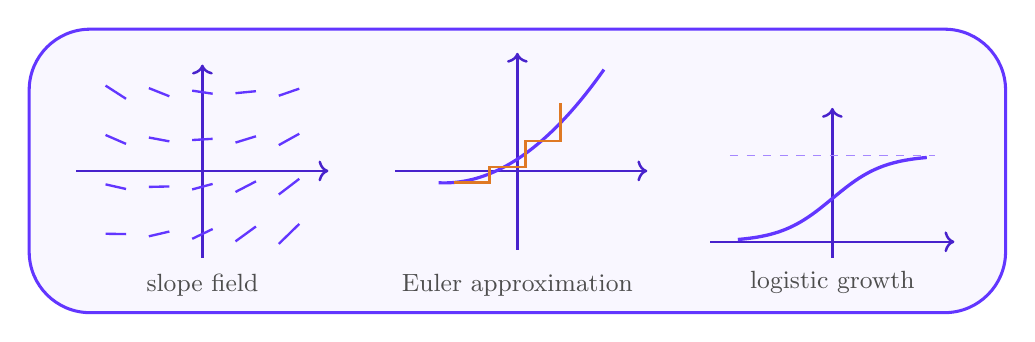
\begin{tikzpicture}[scale=1]
\fill[softlav,rounded corners=22pt] (-6.2,-1.8) rectangle (6.2,1.8);
\draw[novelPurple, line width=1.1pt, rounded corners=22pt] (-6.2,-1.8) rectangle (6.2,1.8);

% left: slope field idea
\begin{scope}[shift={(-4.0,0)}]
\draw[novelPurpleDark, line width=0.9pt, ->] (-1.6,0)--(1.6,0);
\draw[novelPurpleDark, line width=0.9pt, ->] (0,-1.1)--(0,1.35);
\foreach \x in {-1.1,-0.55,0,0.55,1.1}{
  \foreach \y in {-0.8,-0.2,0.4,1.0}{
    \pgfmathsetmacro{\m}{0.45*\x-0.35*\y+0.2}
    \pgfmathsetmacro{\dx}{0.13}
    \pgfmathsetmacro{\dy}{\m*\dx}
    \draw[novelPurple, line width=0.85pt] (\x-\dx,\y-\dy)--(\x+\dx,\y+\dy);
  }
}
\node[text=npgray] at (0,-1.45) {\small slope field};
\end{scope}

% middle: Euler staircase
\begin{scope}[shift={(0,0)}]
\draw[novelPurpleDark, line width=0.9pt, ->] (-1.55,0)--(1.65,0);
\draw[novelPurpleDark, line width=0.9pt, ->] (0,-1.0)--(0,1.5);
\draw[novelPurple, line width=1.15pt, smooth, samples=120, domain=-1.0:1.1]
plot (\x,{0.15 + 0.65*\x + 0.35*\x*\x});
\draw[nporange, line width=1pt] (-0.8,-0.15)--(-0.35,-0.15)--(-0.35,0.05)--(0.1,0.05)--(0.1,0.38)--(0.55,0.38)--(0.55,0.86);
\node[text=npgray] at (0,-1.45) {\small Euler approximation};
\end{scope}

% right: logistic curve
\begin{scope}[shift={(4.0,-0.9)}]
\draw[novelPurpleDark, line width=0.9pt, ->] (-1.55,0)--(1.55,0);
\draw[novelPurpleDark, line width=0.9pt, ->] (0,-0.2)--(0,1.7);
\draw[novelPurpleLine, dashed] (-1.3,1.1)--(1.3,1.1);
\draw[novelPurple, line width=1.2pt, smooth, domain=-1.2:1.2, samples=160]
plot (\x,{1.1/(1+exp(-3*\x))});
\node[text=npgray] at (0,-0.52) {\small logistic growth};
\end{scope}

;
\end{tikzpicture}
}

\newcommand{\proportionalityfigure}{
\begin{center}
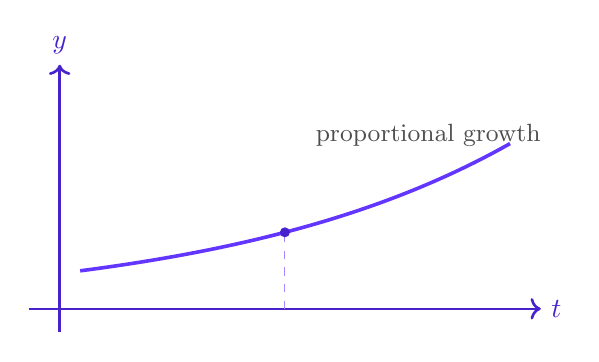
\begin{tikzpicture}[x=1.3cm,y=1.0cm]
\draw[novelPurpleDark, line width=0.95pt, ->] (-0.3,0)--(4.7,0) node[right] {$t$};
\draw[novelPurpleDark, line width=0.95pt, ->] (0,-0.3)--(0,3.1) node[above] {$y$};
\draw[novelPurple, line width=1.3pt, domain=0.2:4.4, samples=160]
plot (\x,{0.45*exp(0.35*\x)});
\draw[novelPurpleLine, dashed] (2.2,0)--(2.2,{0.45*exp(0.35*2.2)});
\fill[novelPurpleDark] (2.2,{0.45*exp(0.35*2.2)}) circle (1.8pt);
\node[text=npgray] at (3.6,2.2) {\small proportional growth};
\end{tikzpicture}
\end{center}
}

\newcommand{\slopefieldbasic}{
\begin{center}
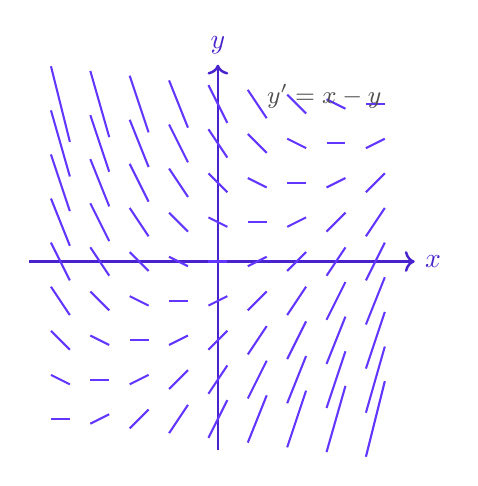
\begin{tikzpicture}[x=1.0cm,y=1.0cm]
\draw[novelPurpleDark, line width=0.9pt, ->] (-2.4,0)--(2.5,0) node[right] {$x$};
\draw[novelPurpleDark, line width=0.9pt, ->] (0,-2.4)--(0,2.5) node[above] {$y$};

\foreach \x in {-2,-1.5,-1,-0.5,0,0.5,1,1.5,2}{
  \foreach \y in {-2,-1.5,-1,-0.5,0,0.5,1,1.5,2}{
    \pgfmathsetmacro{\m}{\x-\y}
    \pgfmathsetmacro{\dx}{0.12}
    \pgfmathsetmacro{\dy}{0.12*\m}
    \draw[novelPurple, line width=0.75pt] (\x-\dx,\y-\dy)--(\x+\dx,\y+\dy);
  }
}
\node[text=npgray] at (1.35,2.1) {\small \(y'=x-y\)};
\end{tikzpicture}
\end{center}
}

\newcommand{\solutioncurveonslopefield}{
\begin{center}
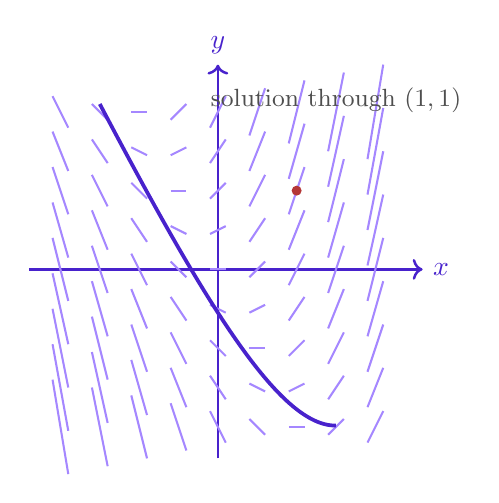
\begin{tikzpicture}[x=1.0cm,y=1.0cm]
\draw[novelPurpleDark, line width=0.9pt, ->] (-2.4,0)--(2.6,0) node[right] {$x$};
\draw[novelPurpleDark, line width=0.9pt, ->] (0,-2.4)--(0,2.6) node[above] {$y$};

\foreach \x in {-2,-1.5,-1,-0.5,0,0.5,1,1.5,2}{
  \foreach \y in {-2,-1.5,-1,-0.5,0,0.5,1,1.5,2}{
    \pgfmathsetmacro{\m}{2*\x+\y}
    \pgfmathsetmacro{\dx}{0.10}
    \pgfmathsetmacro{\dy}{0.10*\m}
    \draw[novelPurpleLine, line width=0.75pt] (\x-\dx,\y-\dy)--(\x+\dx,\y+\dy);
  }
}
\draw[novelPurpleDark, line width=1.35pt, smooth, samples=120, domain=-1.5:1.5]
plot (\x,{0.45*exp(\x)-2*\x-1});
\fill[npred] (1,1) circle (1.8pt);
\node[text=npgray] at (1.5,2.15) {\small solution through \((1,1)\)};
\end{tikzpicture}
\end{center}
}

\newcommand{\eulerfigure}{
\begin{center}
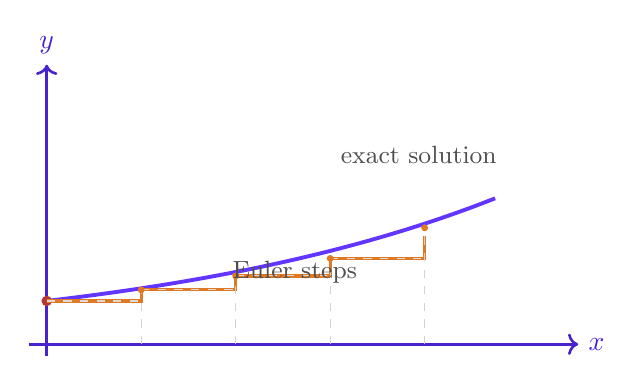
\begin{tikzpicture}[x=1.5cm,y=1.0cm]
    % axes
    \draw[novelPurpleDark, line width=0.95pt, ->] (-0.15,0) -- (4.5,0) node[right] {$x$};
    \draw[novelPurpleDark, line width=0.95pt, ->] (0,-0.15) -- (0,3.55) node[above] {$y$};

    % exact solution
    \draw[novelPurple, line width=1.4pt, smooth, samples=240, domain=0:3.8]
        plot (\x,{0.55*exp(0.32*\x)});

    % start point
    \fill[npred] (0,0.55) circle (1.9pt);

    % Euler polygon
    \draw[nporange, line width=1.15pt]
        (0,0.55) -- (0.8,0.55)
        -- (0.8,0.691)
        -- (1.6,0.691)
        -- (1.6,0.868)
        -- (2.4,0.868)
        -- (2.4,1.090)
        -- (3.2,1.090)
        -- (3.2,1.369);

    % vertical helper lines
    \draw[gray!35, dashed] (0.8,0) -- (0.8,0.691);
    \draw[gray!35, dashed] (1.6,0) -- (1.6,0.868);
    \draw[gray!35, dashed] (2.4,0) -- (2.4,1.090);
    \draw[gray!35, dashed] (3.2,0) -- (3.2,1.369);

    % horizontal helper lines for steps
    \draw[gray!28, dashed] (0,0.55) -- (0.8,0.55);
    \draw[gray!28, dashed] (0.8,0.691) -- (1.6,0.691);
    \draw[gray!28, dashed] (1.6,0.868) -- (2.4,0.868);
    \draw[gray!28, dashed] (2.4,1.090) -- (3.2,1.090);

    % markers
    \fill[nporange] (0.8,0.691) circle (1.25pt);
    \fill[nporange] (1.6,0.868) circle (1.25pt);
    \fill[nporange] (2.4,1.090) circle (1.25pt);
    \fill[nporange] (3.2,1.479) circle (1.25pt);

    % labels
    \node[text=npgray] at (3.15,2.4) {\small exact solution};
    \node[text=npgray] at (2.1,0.92) {\small Euler steps};
\end{tikzpicture}
\end{center}
}

\newcommand{\expfigure}{
\begin{center}
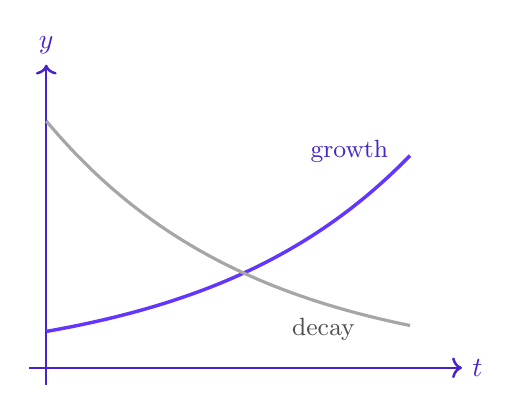
\begin{tikzpicture}[x=1.1cm,y=1.1cm]
\draw[novelPurpleDark, line width=0.9pt, ->] (-0.2,0)--(4.8,0) node[right] {$t$};
\draw[novelPurpleDark, line width=0.9pt, ->] (0,-0.2)--(0,3.5) node[above] {$y$};
\draw[novelPurple, line width=1.25pt, domain=0:4.2, samples=160] plot (\x,{0.42*exp(0.42*\x)});
\draw[gray!70, line width=1.15pt, domain=0:4.2, samples=160] plot (\x,{2.85*exp(-0.42*\x)});
\node[text=novelPurpleDark] at (3.5,2.5) {\small growth};
\node[text=npgray] at (3.2,0.45) {\small decay};
\end{tikzpicture}
\end{center}
}

\newcommand{\logisticfigure}{
\begin{center}
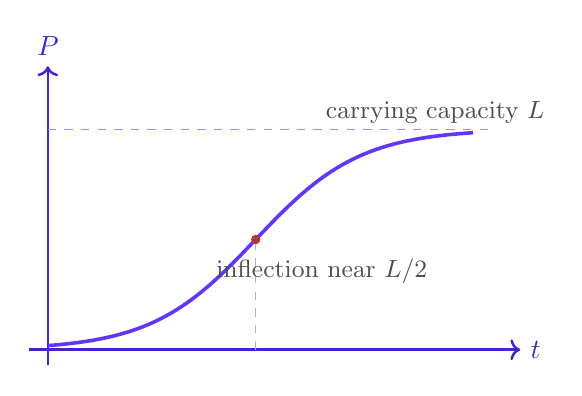
\begin{tikzpicture}[x=1.2cm,y=1.0cm]
\draw[novelPurpleDark, line width=0.9pt, ->] (-0.2,0)--(5.0,0) node[right] {$t$};
\draw[novelPurpleDark, line width=0.9pt, ->] (0,-0.2)--(0,3.6) node[above] {$P$};
\draw[novelPurpleLine, dashed] (0,2.8)--(4.7,2.8);
\draw[gray!60, dashed] (2.2,0)--(2.2,1.4);
\draw[novelPurple, line width=1.3pt, domain=0:4.5, samples=180]
plot (\x,{2.8/(1+exp(-1.8*(\x-2.2)))});
\fill[npred] (2.2,1.4) circle (1.7pt);
\node[text=npgray] at (4.1,3.02) {\small carrying capacity \(L\)};
\node[text=npgray] at (2.9,1.0) {\small inflection near \(L/2\)};
\end{tikzpicture}
\end{center}
}

% =========================================================
\begin{document}

% =========================================================
% Cover Page
% =========================================================
\begin{titlepage}
\centering
\vspace*{2.0cm}

{\fontsize{28}{32}\selectfont\bfseries\color{novelPurpleDark} AP Calculus AB \& BC\par}
\vspace{0.35cm}
{\fontsize{28}{32}\selectfont\bfseries\color{novelPurpleDark} Unit 7: Differential Equations\par}


\vspace{1.0cm}

\decoverfigure

\vfill

\begin{minipage}{0.84\textwidth}
\begin{notebox}{Design Goals for This Revision}
\begin{itemize}
    \item Keep the full Unit 7 sequence from the original handout.
    \item Rebuild the chapter in the same polished Novel Prep style as Units 8, 9, and 10.
    \item Preserve the original examples whenever possible, while correcting wording and solution flow.
    \item Replace unstable or image-dependent diagrams with clean, compile-safe TikZ figures.
    \item Make the chapter strong enough for both first instruction and AP review.
\end{itemize}
\end{notebox}
\end{minipage}

\vfill

{\large\textbf{Novel Prep Learning Center}}\\[0.25em]
{\large J.Z}

\end{titlepage}

\tableofcontents
\newpage

% =========================================================
% Start numbering at Unit 7
% =========================================================
\setcounter{section}{6}
\section{Differential Equations}

\begin{theorybox}{Big Idea}
A differential equation describes how a quantity changes. In Unit 7, students move from:
\[
\text{rate information} \longrightarrow \text{qualitative behavior} \longrightarrow \text{approximation} \longrightarrow \text{explicit models}.
\]
This chapter connects algebraic forms, slope fields, Euler approximations, separable equations, and real-world growth models.
\end{theorybox}

\begin{notebox}{Teaching Philosophy for This Unit}
Students should not treat differential equations as a list of disconnected techniques.  
They should see one coherent question behind the whole unit:

\[
\textit{If I know how something changes, what can I say about the function itself?}
\]

That question appears in symbolic form, graphical form, and modeling form throughout the chapter.
\end{notebox}

\apcheckpoint{
The unit naturally splits into three layers:
\begin{itemize}
    \item \textbf{Representation:} write and interpret differential equations.
    \item \textbf{Qualitative analysis:} slope fields and Euler’s Method.
    \item \textbf{Exact modeling:} separation of variables, exponential models, and logistic models.
\end{itemize}
}

% =========================================================
\unitchapter{Modeling Situations with Differential Equations}

\unitsubtopic{Differential Equations}

\begin{theorybox}{Definition 7.1.1 --- Differential Equations}
A differential equation is an equation involving a function and one or more of its derivatives.  
It describes the relationship between a quantity and its rate of change.
\end{theorybox}

For example, a differential equation may look like
\[
\frac{dy}{dx}=5x.
\]
Here, \(\dfrac{dy}{dx}\) represents the derivative of the function \(y\) with respect to \(x\), so the equation states that the rate of change of \(y\) is \(5x\).

\proportionalityfigure

\begin{theorybox}{Theorem 7.1.1 --- Proportionality}
\begin{enumerate}
    \item If \(a\) is directly proportional to \(b\), then
    \[
    a=kb,
    \]
    where \(k\) is a constant.
    \item If \(a\) is inversely proportional to \(b\), then
    \[
    a=\frac{k}{b},
    \]
    where \(k\) is a constant.
\end{enumerate}
\end{theorybox}

\example{Proportionality questions}
\begin{enumerate}[label=\textbf{(\alph*)}]
    \item The rate of change of \(S\) with respect to \(t\) is inversely proportional to \(x\).
    \item The rate of change of \(A\) with respect to \(t\) is proportional to the product of \(B\) and \(C\).
\end{enumerate}

\solution
\begin{enumerate}[label=\textbf{(\alph*)}]
    \item Because the phrase is \emph{inversely proportional},
    \[
    \frac{dS}{dt}=\frac{k}{x}.
    \]
    \item Because the phrase is \emph{proportional to the product},
    \[
    \frac{dA}{dt}=kBC.
    \]
\end{enumerate}

\example{Cone volume model}
The rate of change of the volume \(V(t)\) of a right circular cone is proportional to the product of the square of its radius \(r\) and its height \(h\).  
Find the differential equation if the cone has height \(8\) inches, radius \(3\) inches, and the volume is changing by \(2\) cubic inches per second.

\solution
The model is
\[
\frac{dV}{dt}=kr^2h.
\]
Substitute the given information:
\[
2=k(3^2)(8)=72k.
\]
So
\[
k=\frac{2}{72}=\frac{1}{36}\approx 0.0277.
\]
Thus the differential equation is
\[
\boxed{\frac{dV}{dt}=0.0277\,r^2h.}
\]

\example{Mr. Kelly running}
Mr. Kelly is running down his street. His position is \(p(t)\), where \(t\) is measured in seconds since the start of his run. His acceleration is proportional to the square root of the time since the start of his run. Find the differential equation if his acceleration is \(0.0277\) km/sec\(^2\) at \(t=3\) seconds.

\solution
Acceleration is proportional to \(\sqrt{t}\), so
\[
\frac{d^2p}{dt^2}=k\sqrt{t}.
\]
Substitute \(t=3\):
\[
0.0277=k\sqrt3.
\]
So
\[
k=\frac{0.0277}{\sqrt3}\approx 0.016.
\]
Hence
\[
\boxed{\frac{d^2p}{dt^2}=0.016\sqrt{t}.}
\]

\example{A second modeling example}
The rate of change of a bacteria population \(B\) with respect to time is directly proportional to the current population and inversely proportional to temperature \(T\). Write a differential equation.

\solution
Direct proportionality to \(B\) gives a factor of \(B\), and inverse proportionality to \(T\) gives a factor of \(\frac{1}{T}\). Therefore
\[
\boxed{\frac{dB}{dt}=k\frac{B}{T}.}
\]

% =========================================================
\unitchapter{Verifying Solutions for Differential Equations}

\begin{notebox}{Guidance for Verifying Solutions}
To verify whether a proposed function satisfies a differential equation:
\begin{enumerate}
    \item Compute the needed derivative(s).
    \item Substitute both the function and derivative(s) into the equation.
    \item Simplify both sides.
    \item If the equation is true, the function is a solution.
\end{enumerate}
\end{notebox}

\begin{theorybox}{Reminder}
Verifying a solution is different from solving a differential equation.  
You are not finding the function from scratch; you are checking whether a given function works.
\end{theorybox}

\example{Verifying a simple solution}
Verify that
\[
y=x^3
\]
is a solution to
\[
\frac{dy}{dx}=3x^2.
\]

\solution
Differentiate:
\[
\frac{dy}{dx}=3x^2.
\]
Substitute into the differential equation:
\[
3x^2=3x^2.
\]
Both sides agree, so
\[
\boxed{y=x^3 \text{ is a solution}.}
\]

\example{Verifying a more complicated solution}
Given
\[
y=3e^{2x}+\cos(4x),
\]
verify whether it satisfies
\[
\frac{y''}{2}+8y=30e^{2x}.
\]

\solution
Differentiate:
\[
y'=6e^{2x}-4\sin(4x),
\]
\[
y''=12e^{2x}-16\cos(4x).
\]
Now substitute:
\[
\frac{y''}{2}+8y
=
\frac{12e^{2x}-16\cos(4x)}{2}+8\left(3e^{2x}+\cos(4x)\right).
\]
Simplify:
\[
6e^{2x}-8\cos(4x)+24e^{2x}+8\cos(4x)=30e^{2x}.
\]
So the equation is satisfied, and
\[
\boxed{y=3e^{2x}+\cos(4x)\text{ is a solution to }\frac{y''}{2}+8y=30e^{2x}.}
\]

\example{From a differential equation to a particular solution}
Given the differential equation
\[
\frac{dy}{dx}=4x+2
\]
with initial condition \((-1,3)\), find the particular solution.

\solution
Integrate both sides:
\[
y=\int (4x+2)\,dx=2x^2+2x+C.
\]
Use the point \((-1,3)\):
\[
3=2(-1)^2+2(-1)+C=2-2+C=C.
\]
So \(C=3\). Therefore
\[
\boxed{y=2x^2+2x+3.}
\]

\example{Checking an exponential solution}
Verify that
\[
y=Ce^{kt}
\]
satisfies
\[
\frac{dy}{dt}=ky.
\]

\solution
Differentiate:
\[
\frac{dy}{dt}=kCe^{kt}.
\]
Since \(y=Ce^{kt}\), we get
\[
\frac{dy}{dt}=ky.
\]
So the function is verified.

% =========================================================
\unitchapter{Sketching Slope Fields}

\unitsubtopic{What a Slope Field Represents}

\begin{theorybox}{Definition 7.3.1 --- Slope Field}
A slope field is a collection of short line segments in the plane, where each segment has slope equal to the value of the differential equation at that point.
\end{theorybox}

Slope fields allow us to visualize solution behavior without explicitly solving the differential equation.

\slopefieldbasic

\example{Sketching a slope field for \(y'=x-y\)}
Sketch a slope field for
\[
y'=x-y
\]
and determine the slopes at \((-1,1)\), \((0,1)\), and \((1,1)\).

\solution
For the differential equation
\[
y'=x-y,
\]
the slope at each point \((x,y)\) is \(x-y\).

At \((-1,1)\):
\[
y'=-1-1=-2.
\]
At \((0,1)\):
\[
y'=0-1=-1.
\]
At \((1,1)\):
\[
y'=1-1=0.
\]
So the corresponding segments are steep negative, less negative, and horizontal.

\example{Identifying horizontal tangent locations}
For
\[
y'=2x+y,
\]
where do horizontal tangent segments occur in the slope field?

\solution
Horizontal tangents occur where
\[
y'=0.
\]
So
\[
2x+y=0
\quad\Longrightarrow\quad
y=-2x.
\]
Thus the horizontal segments lie along the line
\[
\boxed{y=-2x.}
\]

% =========================================================
\unitchapter{Reasoning Using Slope Fields}

\unitsubtopic{Reading Behavior from a Slope Field}

\begin{theorybox}{Qualitative Reasoning Rules}
For a differential equation \(y'=F(x,y)\):
\begin{itemize}
    \item If \(F(x,y)>0\), solution curves are increasing.
    \item If \(F(x,y)<0\), solution curves are decreasing.
    \item If \(F(x,y)=0\), solution curves have horizontal tangents.
    \item Changes in how slopes vary can suggest concavity.
\end{itemize}
\end{theorybox}

\solutioncurveonslopefield

\example{Sketching a solution from a slope field}
Sketch a solution to
\[
y'=2x+y
\]
that passes through \((1,1)\).

\solution
At each point, follow the slope indicated by \(2x+y\).  
Since the initial point is \((1,1)\), the solution must pass through that point and bend according to the surrounding slope segments. The result is a curve that follows the local direction field through \((1,1)\).

\example{A multiple-choice style slope-field question}
Suppose a slope field shows circular-looking solution curves centered at the origin. Which of the following could represent the particular solution satisfying \(y(0)=1\)?

\begin{enumerate}[label=\textbf{(\Alph*)}]
    \item \(y=\dfrac{x}{y}+1\)
    \item \(y=-\dfrac{x}{y}+1\)
    \item \(x^2+(y+1)^2=4\)
    \item \(x^2+y^2=1\)
\end{enumerate}

\solution
A slope field suggesting circles centered at the origin matches
\[
x^2+y^2=1.
\]
Also, \(y(0)=1\) is satisfied by the point \((0,1)\). Therefore the correct answer is
\[
\boxed{\text{D}}.
\]

\example{Must-be-false reasoning}
A slope field is shown for some differential equation. Which statement about a solution \(y=f(x)\) must be false?

\begin{enumerate}[label=\textbf{(\Alph*)}]
    \item The particular solution satisfying \(f(2)=-2\) has a relative minimum at \(x=2\).
    \item The particular solution satisfying \(f(-1)=-1\) is concave up on \(-2<x<1\).
    \item The particular solution satisfying \(f(1)=-2\) is linear.
    \item The particular solution satisfying \(f(-1)=2\) is concave up on \(-3<x<3\).
\end{enumerate}

\solution
From the original class note structure, the intended false statement is
\[
\boxed{\text{B}}.
\]
The reason is that the slope behavior does not consistently support concavity up for that solution across the full interval.

% =========================================================
\unitchapter{Approximating Solutions Using Euler’s Method}

\begin{notebox}{BC ONLY}
Euler’s Method is an AP Calculus BC topic.
\end{notebox}

\begin{theorybox}{Definition 7.5.1 --- Euler’s Method}
If
\[
\frac{dy}{dx}=f(x,y)
\]
and an approximation starts from \((x_0,y_0)\), then with step size \(\Delta x\),
\[
y_{n+1}=y_n+f(x_n,y_n)\Delta x,
\qquad
x_{n+1}=x_n+\Delta x.
\]
\end{theorybox}

\eulerfigure

\begin{summarybox}{How Euler’s Method Works}
Euler’s Method uses the tangent-line slope at the current point to estimate the next point.
\[
\text{new value}=\text{old value}+\text{slope}\times\text{step size}
\]
\end{summarybox}

\example{One-step Euler approximation}
Given
\[
\frac{dy}{dx}=x+y,\qquad y(0)=1,
\]
use Euler’s Method with step size \(\Delta x=0.5\) to approximate \(y(0.5)\).

\solution
Start at \((0,1)\). The slope is
\[
f(0,1)=0+1=1.
\]
Then
\[
y_1=1+(1)(0.5)=1.5.
\]
So
\[
\boxed{y(0.5)\approx 1.5.}
\]

\example{Two-step Euler approximation}
Using the same differential equation
\[
\frac{dy}{dx}=x+y,\qquad y(0)=1,
\]
approximate \(y(1)\) with step size \(\Delta x=0.5\).

\solution
From the previous step:
\[
x_1=0.5,\qquad y_1=1.5.
\]
Now compute the new slope:
\[
f(0.5,1.5)=0.5+1.5=2.
\]
Then
\[
y_2=1.5+(2)(0.5)=2.5.
\]
Thus
\[
\boxed{y(1)\approx 2.5.}
\]

\example{Euler table format}
For
\[
\frac{dy}{dx}=x-y,\qquad y(0)=2,
\]
use Euler’s Method with \(\Delta x=0.5\) for two steps.

\solution
\[
\begin{array}{c|c|c}
x_n & y_n & f(x_n,y_n)=x_n-y_n\\
\hline
0 & 2 & -2\\
0.5 & 1 & -0.5\\
1 & 0.75 & 
\end{array}
\]
So the approximations are
\[
\boxed{y(0.5)\approx 1,\qquad y(1)\approx 0.75.}
\]

% =========================================================
\unitchapter{Finding General Solutions Using Separation of Variables}

\unitsubtopic{Separable Equations}

\begin{theorybox}{Definition 7.6.1 --- Separation of Variables}
A differential equation is separable if it can be written in the form
\[
\frac{dy}{dx}=g(x)h(y).
\]
Then it can be rewritten as
\[
\frac{1}{h(y)}\,dy=g(x)\,dx
\]
so that each variable appears on its own side.
\end{theorybox}

\begin{notebox}{General Procedure}
\begin{enumerate}
    \item Rewrite the equation so all \(y\)-terms are with \(dy\) and all \(x\)-terms are with \(dx\).
    \item Integrate both sides.
    \item Solve algebraically if possible.
\end{enumerate}
\end{notebox}

\example{Basic separation of variables}
Solve
\[
\frac{dy}{dx}=xy.
\]

\solution
Separate variables:
\[
\frac{1}{y}\,dy=x\,dx.
\]
Integrate:
\[
\int \frac{1}{y}\,dy=\int x\,dx
\quad\Longrightarrow\quad
\ln|y|=\frac{x^2}{2}+C.
\]
Exponentiate:
\[
\boxed{y=Ce^{x^2/2}.}
\]

\example{A rational separable equation}
Solve
\[
\frac{dy}{dx}=y(1+x^2).
\]

\solution
Separate:
\[
\frac{1}{y}\,dy=(1+x^2)\,dx.
\]
Integrate:
\[
\ln|y|=x+\frac{x^3}{3}+C.
\]
So
\[
\boxed{y=Ce^{x+x^3/3}.}
\]

\example{A trigonometric separable equation}
Solve
\[
\frac{dy}{dx}=2x\cos y.
\]

\solution
Separate:
\[
\sec y\,dy=2x\,dx.
\]
Integrate:
\[
\int \sec y\,dy=\int 2x\,dx.
\]
So
\[
\ln|\sec y+\tan y|=x^2+C.
\]
This is an implicit general solution:
\[
\boxed{\ln|\sec y+\tan y|=x^2+C.}
\]

% =========================================================
\unitchapter{Finding Particular Solutions Using Initial Conditions and Separation of Variables}

\begin{theorybox}{Particular Solutions}
A general solution contains a constant \(C\).  
A particular solution is found by using an initial condition such as \(y(x_0)=y_0\).
\end{theorybox}

\example{Initial condition with a separable equation}
Given
\[
\frac{dy}{dx}=xy,\qquad y(0)=4,
\]
find the particular solution.

\solution
From the general solution,
\[
y=Ce^{x^2/2}.
\]
Apply \(y(0)=4\):
\[
4=Ce^0=C.
\]
Therefore
\[
\boxed{y=4e^{x^2/2}.}
\]

\example{Particular solution from the original class note}
Given the differential equation
\[
xy\,dx+e^{-x}(y^2-1)\,dy=0,
\]
and the initial condition \(y(0)=1\), find the particular solution.

\solution
Rearrange and separate variables:
\[
e^{-x}(y^2-1)\,dy=-xy\,dx.
\]
Write in separable form:
\[
\frac{y}{y^2-1}\,dy=-xe^x\,dx.
\]
Integrate:
\[
\int \frac{y}{y^2-1}\,dy=-\int xe^x\,dx.
\]
The left side is
\[
\frac12\ln|y^2-1|,
\]
and the right side is
\[
-(x-1)e^x+C.
\]
So an implicit form is
\[
\frac12\ln|y^2-1|=-(x-1)e^x+C.
\]
Because \(y(0)=1\) makes \(y^2-1=0\), this initial value sits on a special solution branch. In fact,
\[
\boxed{y=1}
\]
is itself a constant solution to the original differential equation, since \(y^2-1=0\) makes the left-hand side vanish. Thus the particular solution is
\[
\boxed{y=1.}
\]

\example{Population model}
The rate of change of a population \(N(t)\) is proportional to \(650-N\), where \(t\) is time in years. Initially \(N(0)=300\), and \(N(2)=500\). Find \(N(3)\).

\solution
Write the differential equation:
\[
\frac{dN}{dt}=k(650-N).
\]
Separate variables:
\[
\frac{dN}{650-N}=k\,dt.
\]
Integrate:
\[
-\ln|650-N|=kt+C.
\]
Solve for \(N\):
\[
N=650-Ce^{-kt}.
\]
Use \(N(0)=300\):
\[
300=650-C
\quad\Longrightarrow\quad
C=350.
\]
So
\[
N=650-350e^{-kt}.
\]
Use \(N(2)=500\):
\[
500=650-350e^{-2k}
\quad\Longrightarrow\quad
150=350e^{-2k}
\quad\Longrightarrow\quad
e^{-2k}=\frac{3}{7}.
\]
Thus
\[
e^{-k}=\sqrt{\frac{3}{7}}.
\]
Then
\[
N(3)=650-350e^{-3k}
=650-350\left(\sqrt{\frac{3}{7}}\right)^3.
\]
Numerically,
\[
N(3)\approx 552.
\]
So
\[
\boxed{N(3)\approx 552.}
\]

% =========================================================
\unitchapter{Exponential Models with Differential Equations}

\unitsubtopic{Growth and Decay Models}

\begin{theorybox}{Definition 7.8.1 --- Exponential Growth and Decay}
If the rate of change of a quantity \(y\) is proportional to the quantity itself, then
\[
\frac{dy}{dt}=ky
\]
for some constant \(k\).
\end{theorybox}

\begin{theorybox}{Theorem 7.8.2 --- Exponential Model}
If
\[
\frac{dy}{dt}=ky,
\]
then the general solution is
\[
\boxed{y=Ce^{kt}.}
\]
\begin{itemize}
    \item If \(k>0\), the model is exponential growth.
    \item If \(k<0\), the model is exponential decay.
\end{itemize}
\end{theorybox}

\expfigure

\example{Using an exponential growth model}
A population satisfies
\[
\frac{dP}{dt}=0.06P
\]
with \(P(0)=120\). Find \(P(t)\).

\solution
Since the model is \(\frac{dP}{dt}=kP\), the solution is
\[
P=Ce^{0.06t}.
\]
Use \(P(0)=120\):
\[
120=C.
\]
So
\[
\boxed{P(t)=120e^{0.06t}.}
\]

\example{Using an exponential decay model}
A substance decays according to
\[
\frac{dA}{dt}=-0.3A
\]
with \(A(0)=50\). Find \(A(t)\).

\solution
The solution has the form
\[
A=Ce^{-0.3t}.
\]
Using \(A(0)=50\) gives \(C=50\), so
\[
\boxed{A(t)=50e^{-0.3t}.}
\]

\example{Newton's Law of Cooling}
Let \(y\) represent the temperature (in \(^\circ\!F\)) of an object in a room kept at constant temperature \(60^\circ\). The object cools from \(100^\circ\) to \(90^\circ\) in \(10\) minutes. How much longer will it take to cool to \(80^\circ\)?

\solution
Newton's Law of Cooling gives
\[
\frac{dy}{dt}=k(y-60).
\]
Separate variables:
\[
\frac{1}{y-60}\,dy=k\,dt.
\]
Integrate:
\[
\ln|y-60|=kt+C.
\]
Exponentiate:
\[
y=60+Ce^{kt}.
\]
Use \(y(0)=100\):
\[
100=60+C \quad\Rightarrow\quad C=40.
\]
So
\[
y=60+40e^{kt}.
\]
Use \(y(10)=90\):
\[
90=60+40e^{10k}
\quad\Rightarrow\quad
30=40e^{10k}
\quad\Rightarrow\quad
e^{10k}=\frac34.
\]
Thus
\[
k=\frac{1}{10}\ln\left(\frac34\right)\approx -0.02877.
\]
Now set \(y=80\):
\[
80=60+40e^{kt}
\quad\Rightarrow\quad
20=40e^{kt}
\quad\Rightarrow\quad
e^{kt}=\frac12.
\]
So
\[
t=\frac{\ln(1/2)}{k}\approx 24.1 \text{ minutes}.
\]
Since the object reached \(90^\circ\) at \(10\) minutes, the additional time is
\[
24.1-10=14.1 \text{ minutes}.
\]
Thus it will take about
\[
\boxed{14.1\text{ more minutes}.}
\]

% =========================================================
\unitchapter{Logistic Models with Differential Equations}

\begin{theorybox}{Definition 7.9.1 --- Logistic Differential Equation}
A logistic model describes growth that slows as the population approaches a carrying capacity \(L\):
\[
\frac{dy}{dt}=ky\left(1-\frac{y}{L}\right).
\]
\end{theorybox}

\begin{notebox}{Interpretation}
In the logistic model:
\begin{itemize}
    \item \(y\) is the current population,
    \item \(L\) is the carrying capacity,
    \item \(k\) is a constant,
    \item growth is fastest around \(y=\dfrac{L}{2}\).
\end{itemize}
\end{notebox}

\logisticfigure

\begin{theorybox}{Behavior of the Logistic Model}
For
\[
\frac{dy}{dt}=ky\left(1-\frac{y}{L}\right):
\]
\begin{itemize}
    \item if \(0<y<L\), then \(\dfrac{dy}{dt}>0\), so the population increases;
    \item if \(y>L\), then \(\dfrac{dy}{dt}<0\), so the population decreases;
    \item equilibrium solutions occur at \(y=0\) and \(y=L\).
\end{itemize}
\end{theorybox}

\example{Reading logistic behavior}
Suppose a population satisfies
\[
\frac{dP}{dt}=0.04P\left(1-\frac{P}{500}\right).
\]

\begin{enumerate}[label=\textbf{(\alph*)}]
    \item What is the carrying capacity?
    \item For what population value is the growth rate zero?
    \item When is the growth rate largest?
\end{enumerate}

\solution
\begin{enumerate}[label=\textbf{(\alph*)}]
    \item The carrying capacity is
    \[
    \boxed{500}.
    \]
    \item The growth rate is zero when
    \[
    P=0 \quad \text{or} \quad P=500.
    \]
    \item The logistic growth rate is largest when
    \[
    P=\frac{500}{2}=250.
    \]
\end{enumerate}

\example{Qualitative logistic reasoning}
A population satisfies
\[
\frac{dP}{dt}=kP\left(1-\frac{P}{800}\right),\qquad P(0)=1000.
\]
Determine whether the population initially increases or decreases.

\solution
Because \(P(0)=1000>800\), we have
\[
1-\frac{P}{800}<0.
\]
Thus
\[
\frac{dP}{dt}<0.
\]
So the population initially
\[
\boxed{\text{decreases}.}
\]

\example{Matching a logistic graph}
Which feature best distinguishes a logistic model from a simple exponential growth model?

\solution
A logistic graph levels off at a carrying capacity, while exponential growth continues increasing without bound. The clearest distinguishing feature is
\[
\boxed{\text{horizontal leveling toward a limiting value}.}
\]

% =========================================================
\newpage
\subsection{Unit 7 Summary / Formula Sheet}

\begin{summarybox}{Unit 7 Master Summary Sheet}
\renewcommand{\arraystretch}{1.35}
\begin{tabularx}{\textwidth}{@{}p{0.37\textwidth}X@{}}
\toprule
\textbf{Topic} & \textbf{Key Formula / Idea} \\
\midrule
Differential equation & relates a function to one or more derivatives \\

Direct proportionality & \(a=kb\) \\

Inverse proportionality & \(a=\dfrac{k}{b}\) \\

Verify a solution & differentiate, substitute, simplify \\

Slope field & short segments with slope \(y'=F(x,y)\) \\

Increasing / decreasing from slope field & \(F(x,y)>0\Rightarrow\) increasing,\quad \(F(x,y)<0\Rightarrow\) decreasing \\

Horizontal tangents & \(F(x,y)=0\) \\

Euler’s Method & \(y_{n+1}=y_n+f(x_n,y_n)\Delta x\) \\

Separable equation & \(\dfrac{dy}{dx}=g(x)h(y)\) \\

Separation of variables & \(\dfrac{1}{h(y)}\,dy=g(x)\,dx\) \\

Exponential model & \(\dfrac{dy}{dt}=ky\Rightarrow y=Ce^{kt}\) \\

Growth vs decay & \(k>0\) growth,\quad \(k<0\) decay \\

Logistic model & \(\dfrac{dy}{dt}=ky\left(1-\dfrac{y}{L}\right)\) \\

Carrying capacity & \(L\) \\

Maximum logistic growth rate & at \(y=\dfrac{L}{2}\) \\
\bottomrule
\end{tabularx}
\end{summarybox}

\vspace{1em}

\begin{summarybox}{Strategy Ladder}
\begin{itemize}
    \item If the question says “proportional to,” write a differential equation first.
    \item If a function is given and you are asked whether it works, verify by substitution.
    \item If the graph is a slope field, think increasing / decreasing / horizontal / concavity.
    \item If exact solving is hard but approximation is possible, use Euler’s Method.
    \item If variables can be separated, separate before integrating.
    \item If the rate is proportional to the current amount, think exponential.
    \item If growth slows near a limiting value, think logistic.
\end{itemize}
\end{summarybox}

% =========================================================
\newpage
\subsection{Guided Practice Set}

\begin{practicebox}{Guided Practice A --- Modeling and Verifying}
\begin{enumerate}
    \item Write a differential equation for: “The rate of change of \(Q\) is proportional to \(Q\).”
    \item Write a differential equation for: “The rate of change of \(A\) is inversely proportional to \(t\).”
    \item Verify that \(y=e^{3x}\) satisfies \(\dfrac{dy}{dx}=3y\).
    \item Find the particular solution to \(\dfrac{dy}{dx}=6x-1\) with \(y(0)=4\).
\end{enumerate}
\end{practicebox}

\begin{practicebox}{Guided Practice B --- Slope Fields and Euler}
\begin{enumerate}
    \item For \(y'=x-y\), find the slope at \((2,1)\).
    \item For \(y'=2x+y\), where are the horizontal tangents?
    \item Use one Euler step to approximate \(y(0.5)\) if \(\dfrac{dy}{dx}=x+y\) and \(y(0)=1\).
    \item Explain what a negative slope means on a slope field.
\end{enumerate}
\end{practicebox}

\begin{practicebox}{Guided Practice C --- Separation / Exponential / Logistic}
\begin{enumerate}
    \item Solve \(\dfrac{dy}{dx}=2xy\).
    \item Find the particular solution if \(\dfrac{dy}{dt}=0.5y\) and \(y(0)=8\).
    \item For \(\dfrac{dP}{dt}=0.03P\left(1-\dfrac{P}{600}\right)\), identify the carrying capacity.
    \item For the same model, determine the population at which growth is fastest.
\end{enumerate}
\end{practicebox}

% =========================================================
\newpage
\subsection{Homework / Class Exercises}

\begin{homeworkset}{Homework A --- Modeling and Verifying}
\begin{enumerate}
    \item Write a differential equation for: “The rate of change of \(M\) with respect to \(t\) is proportional to \(M\) and inversely proportional to \(x\).”
    \hwspace

    \item Write a differential equation for: “The acceleration of a particle is proportional to the cube of time.”
    \hwspace

    \item Verify that \(y=\cos x\) satisfies \(y''+y=0\).
    \hwspace

    \item Find the particular solution to \(\dfrac{dy}{dx}=5x-4\) with \(y(1)=2\).
    \hwspace

    \item Verify that \(y=Ce^{kt}\) satisfies \(\dfrac{dy}{dt}=ky\).
\end{enumerate}
\end{homeworkset}

\begin{homeworkset}{Homework B --- Slope Fields and Euler}
\begin{enumerate}
\setcounter{enumi}{5}
    \item For \(y'=x-y\), compute the slope at \((-1,2)\), \((0,2)\), and \((1,2)\).
    \hwspace

    \item For \(y'=3x-y\), determine where horizontal tangent segments occur.
    \hwspace

    \item Use Euler’s Method with \(\Delta x=0.5\) to approximate \(y(1)\) for \(\dfrac{dy}{dx}=x+y\), \(y(0)=2\).
    \hwspace

    \item Use Euler’s Method with \(\Delta x=0.25\) for one step on \(\dfrac{dy}{dx}=2x-y\), \(y(0)=1\).
    \hwspace

    \item A slope field shows slopes changing from positive to negative across a curve. Explain what this may indicate about solution behavior.
\end{enumerate}
\end{homeworkset}
\newpage
\begin{homeworkset}{Homework C --- Separation, Growth, and Logistic Models}
\begin{enumerate}
\setcounter{enumi}{10}
    \item Solve \(\dfrac{dy}{dx}=3xy\).
    \hwspace

    \item Solve \(\dfrac{dy}{dt}=-0.2y\) with \(y(0)=40\).
    \hwspace

    \item A population satisfies \(\dfrac{dP}{dt}=0.05P\left(1-\dfrac{P}{900}\right)\). Find the carrying capacity and the population of maximum growth.
    \hwspace

    \item The temperature of an object in a \(70^\circ\) room cools from \(110^\circ\) to \(90^\circ\) in 8 minutes. Set up the differential equation and find a temperature model.
    \hwspace

    \item The rate of change of a population is proportional to \(400-N\). If \(N(0)=100\), write a general form for the solution.
\end{enumerate}
\end{homeworkset}

% =========================================================
\newpage
\subsection{Answer Key / Instructor Notes}

\begin{enumerate}
    \item
    \[
    \frac{dM}{dt}=k\frac{M}{x}.
    \]

    \item
    \[
    a(t)=kt^3
    \qquad\text{or}\qquad
    \frac{d^2s}{dt^2}=kt^3.
    \]

    \item
    \[
    y=\cos x,\quad y'=-\sin x,\quad y''=-\cos x.
    \]
    So
    \[
    y''+y=-\cos x+\cos x=0.
    \]

    \item
    \[
    y=\int(5x-4)\,dx=\frac52x^2-4x+C.
    \]
    Use \(y(1)=2\):
    \[
    2=\frac52-4+C \Rightarrow C=\frac72.
    \]
    Thus
    \[
    y=\frac52x^2-4x+\frac72.
    \]

    \item Differentiate \(Ce^{kt}\):
    \[
    \frac{dy}{dt}=kCe^{kt}=ky.
    \]

    \item
    \[
    y'=x-y.
    \]
    At \((-1,2)\): \(-3\), at \((0,2)\): \(-2\), at \((1,2)\): \(-1\).

    \item Horizontal tangents occur where
    \[
    3x-y=0 \Rightarrow y=3x.
    \]

    \item Start at \((0,2)\).  
    Step 1:
    \[
    f(0,2)=2,\qquad y_1=2+2(0.5)=3.
    \]
    Step 2:
    \[
    f(0.5,3)=3.5,\qquad y_2=3+3.5(0.5)=4.75.
    \]
    So
    \[
    y(1)\approx 4.75.
    \]

    \item
    \[
    f(0,1)=2(0)-1=-1.
    \]
    So after one step with \(\Delta x=0.25\),
    \[
    y_1=1+(-1)(0.25)=0.75.
    \]

    \item It may indicate that a solution changes from increasing to decreasing, which suggests a local maximum.

    \item
    \[
    \frac{1}{y}\,dy=3x\,dx
    \quad\Rightarrow\quad
    \ln|y|=\frac{3x^2}{2}+C.
    \]
    Hence
    \[
    y=Ce^{3x^2/2}.
    \]

    \item
    \[
    y=Ce^{-0.2t},\qquad y(0)=40 \Rightarrow C=40.
    \]
    So
    \[
    y=40e^{-0.2t}.
    \]

    \item Carrying capacity:
    \[
    900.
    \]
    Fastest growth at
    \[
    \frac{900}{2}=450.
    \]

    \item Set up
    \[
    \frac{dT}{dt}=k(T-70).
    \]
    Then solve similarly to Newton’s Law of Cooling.

    \item
    \[
    \frac{dN}{dt}=k(400-N)
    \Rightarrow
    N=400-Ce^{-kt}.
    \]
    Since \(N(0)=100\), we get
    \[
    C=300,
    \]
    so one form is
    \[
    N=400-300e^{-kt}.
    \]
\end{enumerate}

% =========================================================
\newpage
\subsection{Unit 7 Final Teaching Checklist}

\begin{theorybox}{Before Leaving Unit 7, Students Should Comfortably Handle}
\begin{itemize}
    \item writing differential equations from proportional relationships
    \item verifying whether a proposed function satisfies a differential equation
    \item reading increasing / decreasing / horizontal behavior from slope fields
    \item sketching a solution curve from a slope field
    \item applying Euler’s Method step by step
    \item separating variables and solving basic separable equations
    \item using initial conditions to determine particular solutions
    \item distinguishing exponential growth from exponential decay
    \item interpreting carrying capacity and equilibrium values in logistic models
    \item identifying where logistic growth is largest
\end{itemize}
\end{theorybox}

\vfill
\begin{center}
{\Large\color{novelPurpleDark}\textbf{End of Unit 7}}\\[0.35em]
{\large Differential Equations}
\end{center}

\end{document}